\subsolution{Фрикционная сварка}{3.5}

Сперва определим выделяющуюся мощность от трения. На единицу площадки $dS$ мощность тепловых потерь равна

\begin{eq}[points=0.3]
dP = \mu\cdot p dS\cdot \omega r,
\end{eq}

\criterion[type=remark]{Балл ставится и при записи $\omega r\Leftrightarrow v$ или $dS\Leftrightarrow2\pi rdr\Leftrightarrow rd\varphi dr$ или $pdS\Leftrightarrow dN$. За $P=\mu N v$ или прочие \textbf{не}инфинитезимальные записи балл не ставится.}

где $r<R$ --- переменный радиус. Так как $dS = 2\pi r dr$, интегрированием получаем

\begin{eq}[points=0.5]
P = \frac23 \mu p\omega \pi R^3.
\end{eq}

\criterion[type=penalty, points=-0.3]{Вместо коэффициента $2/3$ стоит $1$ либо $1/2$. Если за \eqref{2} стоит \textbf{не}нулевой балл, то ошибка в \eqref{2} должна быть учтена в \eqref{6}, \eqref{7}, и \eqref{10}}

Выделенная теплота распределяется вдоль осей двух цилиндров. В дальнейшем задача превращается в анализ распределения температуры $T(x)$ от координаты $x$ вдоль оси, и приравнивание $T=T^*$ в центре сварки. Рассмотрим половину мощности $P/2$, уходящую, например, в $x>0$, поскольку очевидно, что $T(-x)=T(x)$. В данной задаче два механизма теплопередачи: теплопроводность Фурье

\begin{eq}
[
    points=0.3,
    tail={. Знак минус необязателен, однако это влияет на наличие знака минус в \eqref{5}.}
]
j = -\kappa \pi R^2\frac{dT}{dx},
\end{eq}
который показывает поток тепла $j$ через площадь $S=\pi R^2$, и теплоотдача в воздух (закон Ньютона--Рихмана):

\begin{eq}[points=0.3]
dq = \alpha\cdot 2\pi R dx\cdot(T-T_0).
\end{eq}
По уравнению непрерывности тепловой энергии для $x\ne0$ для диска толщиной $dx$,

\begin{eq}
[
    points=0.3,
    tail={. Отсутствие знака минус \textbf{не} принимается, если это приводит к несоответствию в знаках минус между \eqref{3} и этим уравнением.}
]
j(x+dx)-j(x)=dj=-dq.
\end{eq}

\begin{figure}[!ht]
\centering
\resizebox{0.25\linewidth}{!}{%
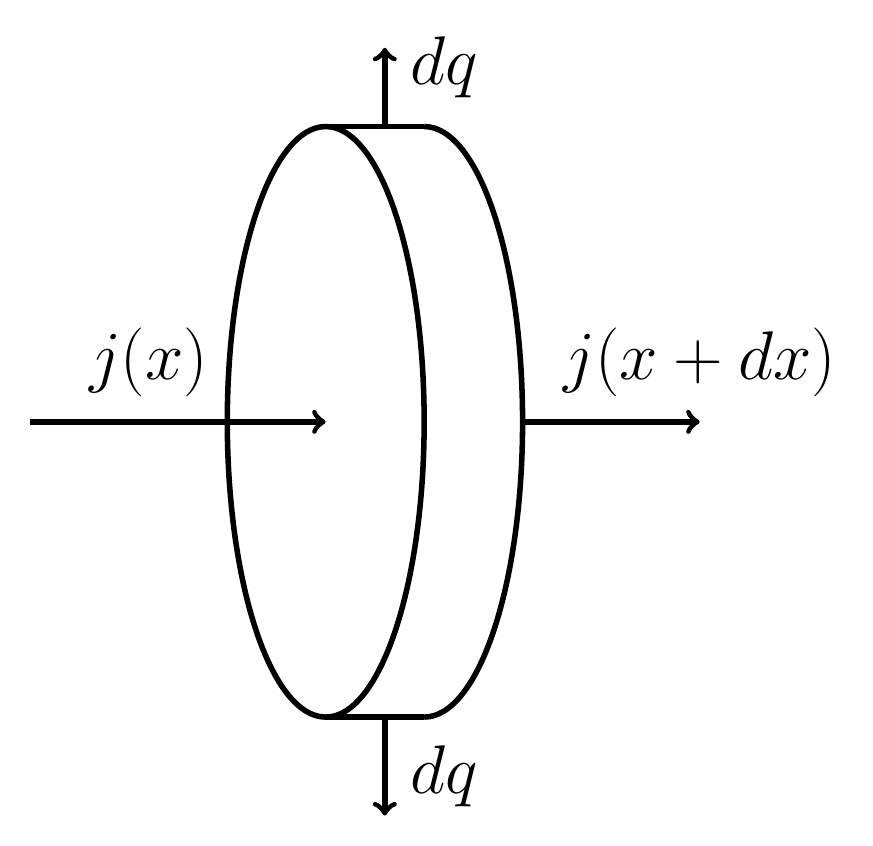
\begin{tikzpicture}[line width=2pt, font=\Huge]
    \draw (13.75, 13.75) ellipse (1.25 and 3.75);
    \draw (15, 17.5) arc (90:-90:1.25 and 3.75);
    \draw (13.75, 17.5) -- (15, 17.5);
    \draw (13.75, 10.0) -- (15, 10.0);
    \draw [->] (10,13.75) -- (13.75,13.75);
    \draw [->] (16.25,13.75) -- (18.5,13.75);
    \node at (11.5,14.5) {$j(x)$};
    \node at (18.5,14.5) {$j(x+dx)$};
    \draw [->] (14.5,17.5) -- (14.5,18.5);
    \draw [->] (14.5,10) -- (14.5,8.75);
    \node at (15.25,18.25) {$dq$};
    \node at (15.25,9.25) {$dq$};
\end{tikzpicture}
}%
\end{figure}

Собирая \eqref{3}--\eqref{4} в \eqref{5}, получаем уравнение вида

\begin{eq}[points=0.2]
\frac{d^2T}{dx^2} = \frac{2\alpha}{\kappa R}(T-T_0).
\end{eq}

Это --- ``уравнение колебаний'', но с отрицательным квадратом угловой частоты. Используя математическую подсказку и получая

\begin{eq}[points=0.2]
\lambda=\sqrt\frac{2\alpha}{\kappa R},
\end{eq}

видим, с учётом симметрии относительно $x=0$, что общее решение должно иметь вид

\begin{eq}[points=0.4]
T(x)=T_0+A\exp\ab(-\lambda|x|)
\end{eq}

\criterion[type=remark]{Модуль необязателен. Принимается если вместо $T_0$ стоит произвольная \textbf{ненулевая} константа. В остальных случаях балл не ставится.}

с некоторой константой $A$, которую нужно найти. Здесь отрицательный $\lambda$ отброшен, так как иначе положительная экспонента улетела бы в бесконечность. В целом, анализ обоих случаев $x>0$ и $x<0$ от участника не требуется, так как важно лишь правильно найти граничное условие. Мы имеем

\begin{eq}[points=0.3]
j(0)=\frac P2.
\end{eq}

(Более правильно говоря, $j(0^+)=+P/2$ и $j(0^-)=-P/2$). Решая с учётом $T(0)=T^*$, получаем

$$
\frac P2 = \kappa \pi R^2 \cdot \ab(\sqrt{\frac{2\alpha}{\kappa R}}\cdot A)\implies  A = \frac{P}{2\pi R\sqrt{2\kappa\alpha R}} = T^* - T_0,
$$

\begin{eq}[points=0.5, numpoints=0.2]
\omega = \frac3{\mu pR}\sqrt\frac{2\kappa\alpha }R\cdot(T^*-T_0)=\qty{51.0}{\radian\per\s}.
\end{eq}

\criterion[type=remark]{Переноса ошибки в численных расчётах нет}

Это немногим менее 500 оборотов в минуту. Реалистичный диапазон составляет от 400 до 1500 оборотов в минуту. Конечно, более реалистичные механизмы фрикционной сварки не могут быть квазистационарными, однако данная модель неплохо получает результат в реалистичном диапазоне способом учёта основных механизмов данного процесса.
